\documentclass[11pt, landscape]{article}
\usepackage[english]{babel}
\usepackage{graphicx}
\usepackage{xcolor}
\usepackage{tikz}
\usetikzlibrary{shapes,arrows,positioning}
\pgfrealjobname{organigram}
\pagestyle{empty}
\begin{document}


\begin{figure}[!h]  
\beginpgfgraphicnamed{orga}
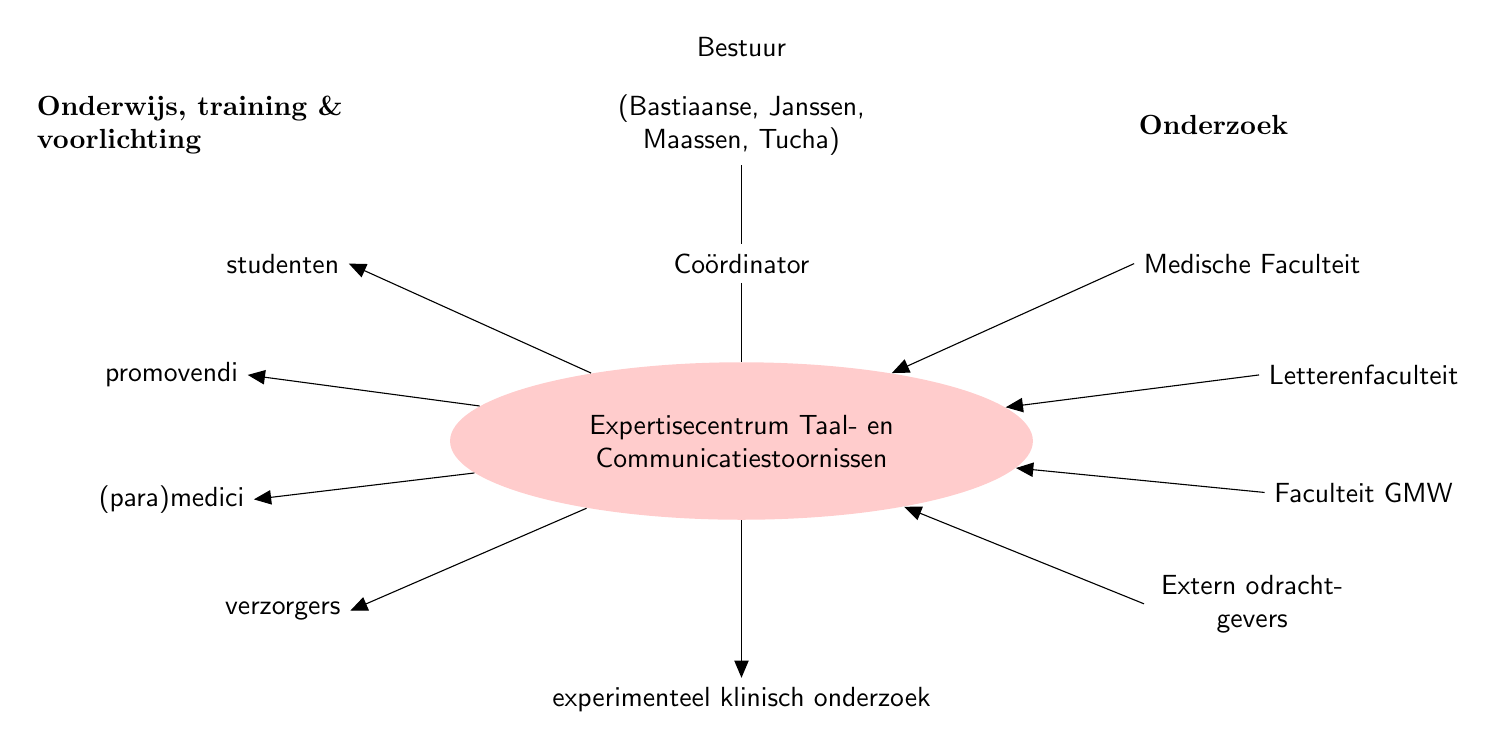
\begin{tikzpicture}[font=\sf]
\begin{centering}

\node(bestuur){Bestuur};
\node(bestuur2)[below of =bestuur, text width = 4cm, text centered]{(Bastiaanse, Janssen, Maassen, Tucha)};
\node(co)[below =1cm of bestuur2]{Co\"ordinator};
\node(etc) [below =1cm of co, ellipse, fill=red!20, minimum height = 2cm, text width = 5cm, text centered]{Expertisecentrum Taal- en Communicatiestoornissen}; 
\node(klinisch)[below =2cm of etc, text width = 5cm, text badly centered]{experimenteel klinisch onderzoek};

\node(otv)[font=\bf, left =2.6cm of bestuur2, text width = 4.1cm]{Onderwijs, training \& voorlichting};

\node(stud)[left =4cm of co]{studenten};
\node(prom)[below left of =stud, node distance = 2cm]{promovendi};
\node(med)[below =1cm of prom]{(para)medici};
\node(verzorg)[below right of =med, node distance = 2cm]{verzorgers};

\node(ond)[font=\bf, right =2.8cm of bestuur2]{Onderzoek};

\node(medF)[right =4cm of co]{Medische Faculteit};
\node(let)[below right of =medF, node distance = 2cm]{Letterenfaculteit};
\node(gmw)[below =1cm of let]{Faculteit GMW};
\node(ext)[below left of =gmw, text width = 2.5cm, node distance = 2cm, text centered]{Extern odrachtgevers};

\path[draw](bestuur2)--(co);
\path[draw] (co)--(etc);
\draw[-triangle 45](etc)--(klinisch);

\foreach \x in {stud, prom, med, verzorg}
	\draw[-triangle 45](etc)--(\x.east);

\foreach \x in {medF, let, gmw, ext}
	\draw[triangle 45-](etc)--(\x.west);







\end{centering}
\end{tikzpicture}
\endpgfgraphicnamed
\end{figure}
\end{document}